\Problem{Visual Dot Product Practice}{\VisDotProdPracA}{
(a) If $ \vec{A}\cdot\vec{B} = 0 $, can you conclude that one of the vectors has zero magnitude? Explain.
}
\Solution{\VisDotProdPracASol}{No. The vectors $ \vec{A} $ and $ \vec{B} $ could be perpendicular to each other.}
\ProblemSub{\VisDotProdPracB}{
(b) For each pair of vectors, is the sign of $ \vec{A}\cdot\vec{B} $ positive (+), negative ($ - $), or zero (0)?
}
\ProblemFig{\VisDotProdPracBFig}{
\centering
\if\GrayProb1
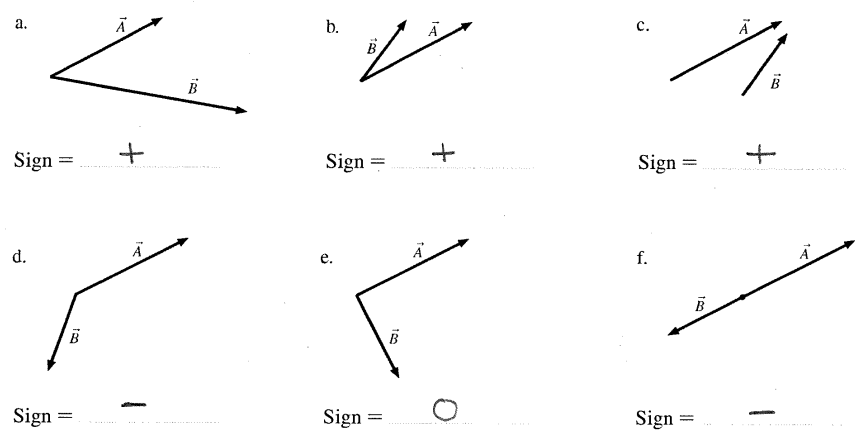
\includegraphics[scale=0.45]{\FileDepth/Activities/Visual_Dot_Product_Practice/Vectors_to_Dots_Solution.png}
\else
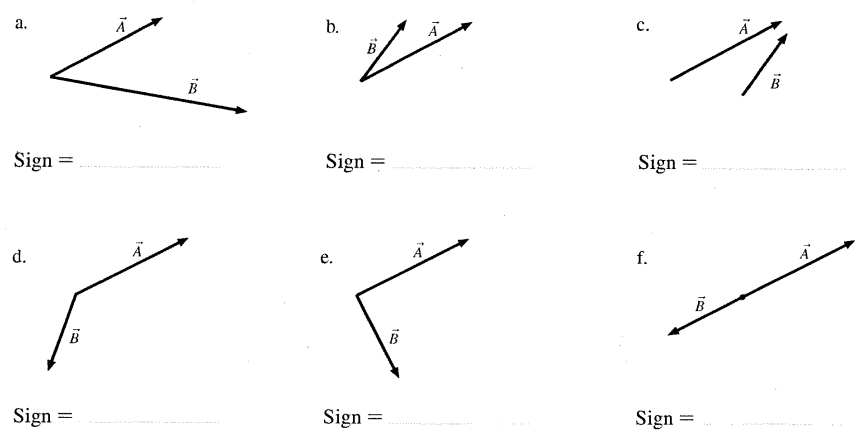
\includegraphics[scale=0.45]{\FileDepth/Activities/Visual_Dot_Product_Practice/Vectors_to_Dots_Blank.png}
\fi
}
\ProblemSub{\VisDotProdPracC}{
(c) Each of the diagrams below shows a vector $ \vec{A} $. Draw and label a vector $ \vec{B} $ that will cause $ \vec{A}\cdot\vec{B} $ to have the sign indicated.
}
\ProblemFig{\VisDotProdPracCFig}{
\centering
\if\GrayProb1
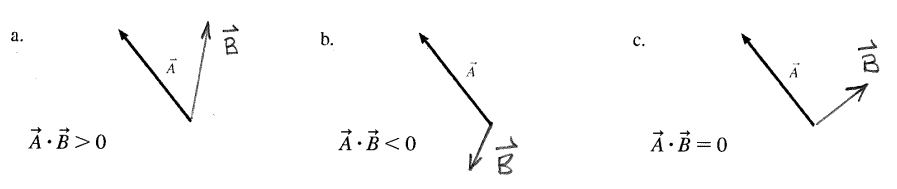
\includegraphics[scale=0.45]{\FileDepth/Activities/Visual_Dot_Product_Practice/Dots_to_Vectors_Solution.png}
\else
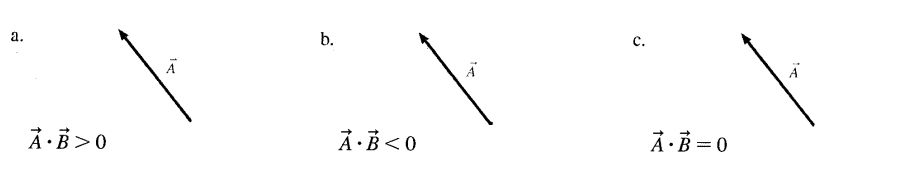
\includegraphics[scale=0.45]{\FileDepth/Activities/Visual_Dot_Product_Practice/Dots_to_Vectors_Blank.png}
\fi
}